\documentclass[twocolumn]{article}
% Language setting
% Replace `english' with e.g. `spanish' to change the document language
\usepackage[spanish]{babel}
\addto{\captionsspanish}{\renewcommand{\abstractname}{Abstract}}
% Set page size and margins
% Replace `letterpaper' with `a4paper' for UK/EU standard size
\usepackage[letterpaper,top=2cm,bottom=2cm,left=2cm,right=2cm,marginparwidth=1.75cm]{geometry}

% Useful packages
\usepackage{amsmath}
\usepackage{dirtytalk}
\usepackage{cancel}
\usepackage{graphicx}
\usepackage[colorlinks=true, allcolors=blue]{hyperref}
\usepackage{blindtext}
\usepackage{multicol}
\usepackage{abstract}
\usepackage{float}

\title{Clasificación de alimentos con ResNet50}
\author{José Pablo Martínez Valdivia}

\begin{document}

\twocolumn[
  \maketitle
  \begin{onecolabstract}
    Convolutional Neural Networks (CNNs) have become the state-of-the-art approach for solving computer vision tasks, thanks to their ability to automatically learn relevant features from images. This study focuses on the classification of food images using a ResNet50 model. The dataset was curated and preprocessed to ensure balance and quality, while data augmentation was applied to increase variability. Two training approaches were compared: training the model from scratch and leveraging Transfer Learning with a pre-trained ResNet50 backbone.
  \end{onecolabstract}
]

\section{Introducción}
Este trabajo se centra en la clasificación de imágenes de alimentos por medio de redes neuronales convolucionales (CNN, por sus siglas en inglés). Utilizamos el modelo ResNet50, una arquitectura reconocida por ser pionera en el uso de conexiones residules, las cuales permitieron mitigar problemas en redes neuronales profundas.

El objetivo principal de este proyecto es comparar dos enfoques de entrenamiento: el entrenamiento desde cero y el uso de Transfer Learning con pesos preentrenados. A través de estos experimentos, se espera obtener una visión clara sobre las ventajas y limitaciones de cada método.

\section{ETL} 
\subsection{Extracción} El dataset utilizado como base fue \say{Food Image Classification}, provisto por la plataforma Kaggle \cite{datasetsrc}, el cual contenía inicialmente 23,837 fotos de 34 clases correspondientes a distintos platillos. Estas imágenes fueron obtenidas de varias páginas de Google Imágenes, según se menciona en la descripción del dataset.

El uso de todas las imágenes resultó problemático durante el entrenamiento debido a las limitaciones de memoria de la tarjeta gráfica empleada. Por esta razón, fue necesario reducir el dataset a 15 clases, con un máximo de 400 imágenes por clase. Las clases seleccionadas fueron:

\begin{itemize} 
    \setlength\itemsep{-0.5em}
    \item apple pie
    \item baked potato
    \item burger
    \item cheesecake
    \item crispy chicken
    \item donut
    \item fried rice
    \item fries
    \item hot dog
    \item ice cream
    \item omelette
    \item pizza
    \item sandwich
    \item sushi
    \item taco
\end{itemize}

Los directorios de estas clases fueron trasladados al nuevo dataset, y se realizó una selección manual de las imágenes de cada clase. Esto se llevó a cabo con el objetivo de eliminar aquellas imágenes que habían sido asignadas erróneamente a alguna categoría. Como resultado, el dataset final consistió en 5,481 imágenes.

Es importante destacar que el dataset original no contenía una cantidad balanceada de imágenes por clase. Por lo tanto, dependiendo de la disponibilidad de imágenes para cada categoría, se seleccionaron entre 300 y 400 imágenes por clase. Esto permitió balancear parcialmente la variabilidad del dataset y reducir los sesgos hacia clases específicas.

\subsection{Aumentación de datos} 
Dado que las fotos fueron obtenidas de Google Imágenes, se observó que muchas de ellas provienen de productos cuyos fotógrafos tienden a capturarlas con una orientación similar. Para incrementar la variabilidad en estas clases, se aplicaron técnicas de aumentación de datos, como rotaciones y escalados aleatorios.

\subsection{Transformación} 
Con el objetivo de evitar la necesidad de realizar transformaciones durante el entrenamiento, se decidió aplicar previamente todas las transformaciones requeridas y guardar los tensores resultantes en archivos serializados.

\section{Marco Teórico}
\subsection{Capas convolucionales}
La tarea de clasificación de imágenes requiere bloques convolucionales capaces de aprender características espaciales presentes en una imagen. Esto se logra mediante la convolución, una operación que consiste básicamente en una suma ponderada entre un arreglo multidimensional de tamaño fijo, conocido como kernel con los píxeles y canales de la imagen. Este kernel se centra sucesivamente en cada uno de los píxeles para realizar la operación de convolución (\ref{fig:convdiag}).

\begin{figure}[!ht]
\centering
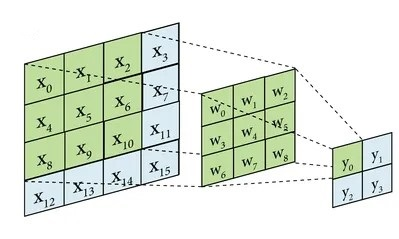
\includegraphics[width=0.4\textwidth]{assets/conv.jpg}
\caption{Operación de convolución \cite{matrixconvsource}.}
\label{fig:convdiag}
\end{figure}

La convolución permite generar mapas de activación, en los cuales los elementos del kernel actúan como pesos que activan o suprimen el resultado de la salida. En los modelos de visión, estos mapas inicialmente detectan características simples como bordes o colores. Sin embargo, después de varias capas convolucionales, el modelo es capaz de identificar patrones más complejos, como rostros u otros objetos específicos.

\subsection{ResNet}
El cálculo de la pérdida que se realiza en la última capa de una red neuronal durante el entrenamiento se propaga hacia atrás multiplicándose por las derivadas de las capas de activación y los pesos de la red para calcular el gradiente y ajustar estos parámetros. En redes profundas, este proceso puede causar que el gradiente se reduzca o aumente excesivamente a través de las capas, lo que da lugar al problema de vanishing o exploding gradients.

La arquitectura ResNet introduce un bloque residual (\ref{fig:skip}) que mitiga este problema. Este bloque incorpora una conexión denominada skip, que consiste en sumar la salida de un bloque de capas convolucionales con el tensor de entrada. Esto permite que el gradiente fluya libremente hacia capas anteriores durante el ajuste de pesos, reduciendo significativamente el riesgo de pérdida o aumento excesivo del gradiente.

\begin{figure}[!ht]
\centering
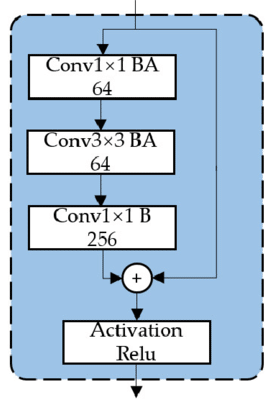
\includegraphics[width=0.2\textwidth]{assets/ResNet50Skip.png}
\caption{Conexión skip \cite{resnet50research}.}
\label{fig:skip}
\end{figure}

Cada bloque residual reduce las dimensiones de ancho y alto de la imagen, mientras incrementa el número de canales. Para lograr esto, es necesario un bloque de proyección (\ref{fig:projblock}), que emplea una convolución de 1x1 en lugar de la conexión skip, igualando los canales de entrada con los de salida.

\begin{figure}[!ht]
\centering
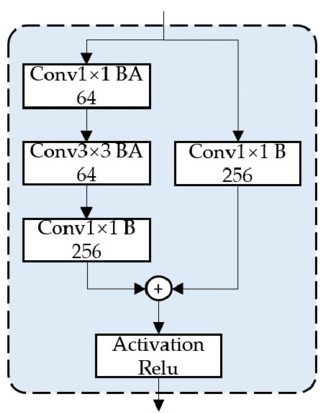
\includegraphics[width=0.2\textwidth]{assets/ResNet50Proj.png}
\caption{Bloque de proyección \cite{resnet50research}.}
\label{fig:projblock}
\end{figure}

La arquitectura seleccionada para la clasificación fue ResNet50 (\ref{tab:resnet50arch}), que cuenta con 50 capas convolucionales en su backbone para la extracción de características de las imágenes. Esta red finaliza con capas densas (\ref{tab:classifier}) que generan una salida correspondiente a cada una de las clases.

\begin{table}[h!]
\centering
\label{tab:classifier}
\begin{tabular}{|l|c|c|c|}
\hline
    \textbf{Capa} & \textbf{Salida}  & \textbf{Details} \\ \hline
    Flatten               & (2048)               & - \\ \hline
    Dense                 & (256)                & ReLU Activation \\ \hline
    Dense                 & (\textit{NUM CLASES})  & - \\ \hline
\end{tabular}
\caption{Clasificador}
\end{table}

\section{Modelado}
\subsection{Entrenamiento con pesos aleatorios}
El dataset fue dividido en un 80\% para datos de entrenamiento y un 20\% para validación. Se utilizó el optimizador \textit{Adam} para ajustar los pesos y la función de pérdida \textit{Entropía cruzada} Además, se implementó un programador \textit{scheduler} para reducir progresivamente la tasa de aprendizaje cada cierto intervalo de tiempo \textit{step\_size} en proporción al parámetro \textit{gamma}, lo cual ayuda a estabilizar el ajuste de los pesos.

Asimismo, se utilizó la técnica de early stopping para finalizar el entrenamiento de forma anticipada si la pérdida no mejoraba después de un número máximo de épocas consecutivas. El modelo fue entrenado con los siguientes hiperparámetros:

\begin{itemize}
    \setlength\itemsep{0.1em}
    \item taza de aprendizaje: 0.01
    \item step\_size (scheduler): 10
    \item gamma (scheduler): 0.5
    \item paciencia 30
    \item épocas máximas: 100
    \item tamaño de lote: 32
\end{itemize}

\subsection{Evaluación con pesos aleatorios}
El modelo finalizó el entrenamiento de forma anticipada en la época 40. Los pesos con el mejor desempeño en el conjunto de validación lograron una pérdida de 1.4032 y una precisión del 55.54\%.

En las gráficas de entrenamiento (\ref{fig:train1loss}) se observa un claro sobreajuste del modelo, evidenciado por la diferencia significativa entre la precisión en el conjunto de entrenamiento y el de validación. Asimismo, al analizar la matriz de confusión (\ref{fig:conf1}), se aprecia que el modelo tiene dificultades para diferenciar ciertas clases.

\begin{figure}[!ht]
\centering
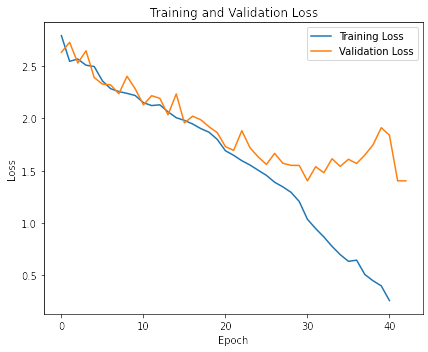
\includegraphics[width=0.4\textwidth]{assets/trainmodel1loss.png}
\caption{Pérdida modelo 1.}
\label{fig:train1loss}
\end{figure}

\begin{figure}[!ht]
\centering
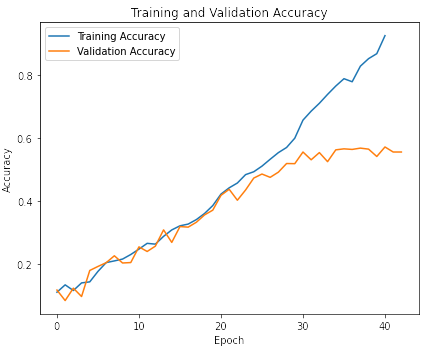
\includegraphics[width=0.4\textwidth]{assets/trainmodel1acc.png}
\caption{Precisión modelo 1.}
\label{fig:train1acc}
\end{figure}

Este desempeño limitado puede atribuirse a la variabilidad del dataset y las características de las clases. Es posible que el modelo encuentre dificultades para identificar y generalizar patrones debido al dominio específico del dataset y al reducido número de imágenes y cantidad de clases.

\begin{figure}[!ht]
\centering
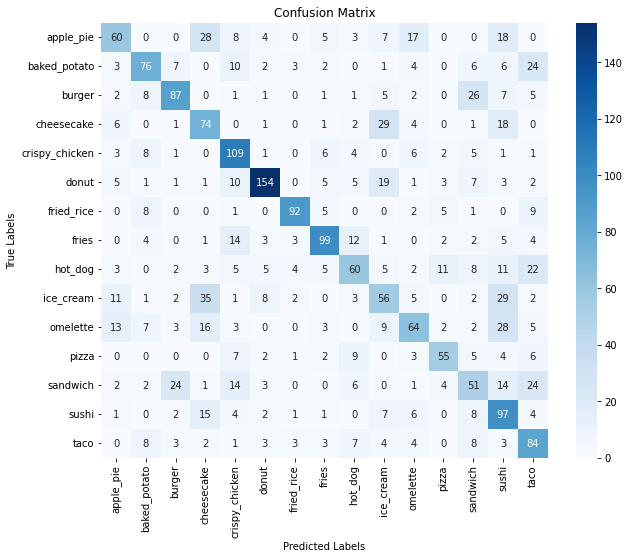
\includegraphics[width=0.45\textwidth]{assets/confmodel1.png}
\caption{Matriz de confusión modelo 1.}
\label{fig:conf1}
\end{figure}

\subsection{Entrenamiento con Transfer Learning} 
Se utilizó la arquitectura ResNet50 previamente entrenada con el conjunto de datos ImageNet. Los pesos del backbone fueron congelados, de manera que únicamente se entrenó el clasificador (\ref{tab:classifier}). El entrenamiento se llevó a cabo utilizando los siguientes hiperparámetros:
\begin{itemize}
    \setlength\itemsep{0.1em}
    \item taza de aprendizaje: 0.001
    \item step\_size (scheduler): 10
    \item gamma (scheduler): 0.5
    \item paciencia 10
    \item épocas máximas: 50
    \item tamaño de lote: 32
\end{itemize}

\subsection{Evaluación del Transfer Learning} El modelo finalizó de forma anticipada en la época 21, logrando una pérdida de 0.2989 y una precisión del 92.29\%. Este resultado refleja una capacidad predictiva sobresaliente en el conjunto de datos de validación y una mejora significativa en comparación con el modelo sin pesos preentrenados.

Además, la matriz de confusión (\ref{fig:conf2}) muestra una reducción notable en la confusión entre las clases, lo que evidencia que el modelo puede diferenciar mejor entre las categorías presentes en el conjunto de datos de validación.

\begin{figure}[!ht]
\centering
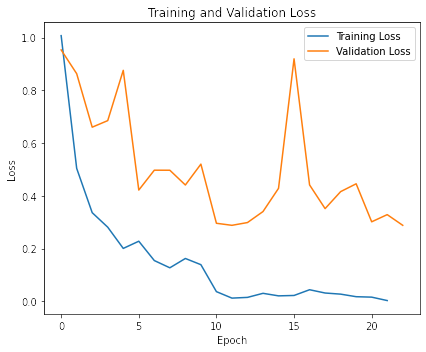
\includegraphics[width=0.4\textwidth]{assets/trainmodel2loss.png}
\caption{Pérdida modelo 2.}
\label{fig:train2loss}
\end{figure}

\begin{figure}[!ht]
\centering
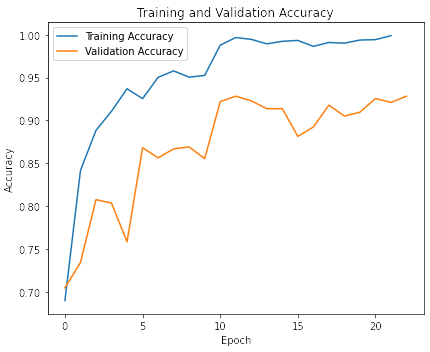
\includegraphics[width=0.4\textwidth]{assets/trainmodel2acc.png}
\caption{Precisión modelo 2.}
\label{fig:train2acc}
\end{figure}
    
\begin{figure*}[!ht]
\centering
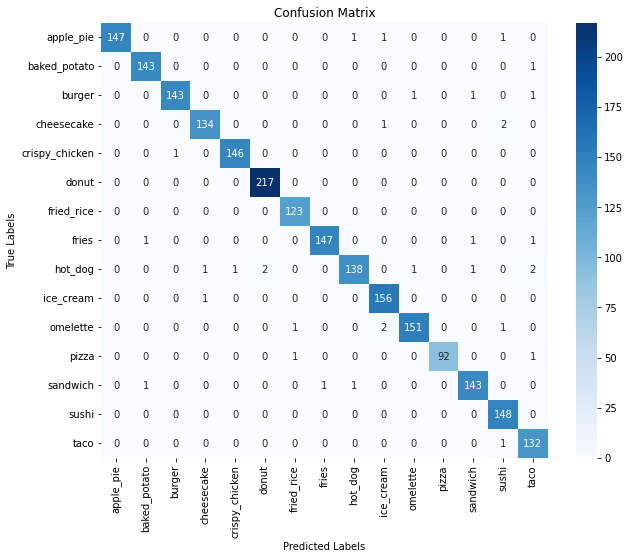
\includegraphics[width=0.45\textwidth]{assets/confmodel2.png}
\caption{Matriz de confusión modelo 2.}
\label{fig:conf2}
\end{figure*}


\section{Conclusión}
Las redes neuronales convolucionales representan el estado del arte en tareas de visión computacional, gracias a su capacidad para extraer características espaciales en imágenes. Este estudio demuestra la importancia de utilizar un backbone preentrenado, como ResNet50, para mejorar el desempeño en tareas de clasificación de imágenes, especialmente cuando se trabaja con conjuntos de datos limitados o específicos.

El uso de Transfer Learning permitió alcanzar una precisión significativamente mayor en comparación con el entrenamiento desde cero, resaltando la ventaja de aprovechar conocimientos previamente adquiridos por modelos más grandes. Esto demuestra la importanci de contar con características bien aprendidas en las primeras capas del modelo para abordar problemas de clasificación en imágenes.

\begin{table*}[h!]
\centering
\label{tab:resnet50arch}
\begin{tabular}{|l|c|c|c|}
\hline
\textbf{Capa} & \textbf{Salida} & \textbf{Detalles} \\ \hline
    Input                 & (224, 224, 3)        & Imagen RGB \\ \hline
    Conv2D                & (112, 112, 64)       & $7\times7$, stride=2 \\ \hline
    BatchNorm2D           & (112, 112, 64)       & - \\ \hline
    ReLU                  & (112, 112, 64)       & - \\ \hline
    MaxPooling2D          & (56, 56, 64)         & $2\times2$, stride=2 \\ \hline
    Residual (Capa 1)     & (56, 56, 256)        & 3 capas    \\ \hline
    Residual (Capa 2)     & (28, 28, 512)        & 4 capas    \\ \hline
    Residual (Capa 3)     & (14, 14, 1024)       & 6 capas    \\ \hline
    Residual (Capa 4)     & (7, 7, 2048)         & 3 capas    \\ \hline
    Global Avg Pooling    & (1, 1, 2048)         & Pooling adaptativo \\ \hline
\end{tabular}
\caption{Backbone ResNet50}
\end{table*}


\begin{table*}[h!]
\centering
\label{tab:residual_block}
\begin{tabular}{|l|c|c|c|}
\hline
    \textbf{Capa} & \textbf{Salida}  & \textbf{Details} \\ \hline
    Conv2D                & (H, W, inChannels)   & $1\times1$, stride=1 \\ \hline
    BatchNorm2D           & (H, W, inChannels)   & - \\ \hline
    ReLU                  & (H, W, inChannels)   & - \\ \hline
    Conv2D                & (H, W, inChannels)   & $3\times3$, stride=1 \\ \hline
    BatchNorm2D           & (H, W, inChannels)   & - \\ \hline
    ReLU                  & (H, W, inChannels)   & - \\ \hline
    Conv2D                & (H, W, outChannels)  & $1\times1$, stride=1 \\ \hline
    BatchNorm2D           & (H, W, outChannels)  & - \\ \hline
    Residual Connection   & (H, W, outChannels)  & Identidad o proyección \\ \hline
    ReLU                  & (H, W, outChannels)  & - \\ \hline
\end{tabular}
\caption{Bloque Residual ResNet50}
\end{table*}


\begin{thebibliography}{9}
\bibitem{datasetsrc}
Food Image Classification Dataset. (2023, 4 julio). Kaggle. https://www.kaggle.com/datasets/
harishkumardatalab/food-image-classification-dataset?select=Food+Classification+dataset

\bibitem{matrixconvsource}
Sahoo, S. (2024, 22 enero). 2D Convolution using Python \& NumPy - Analytics Vidhya - Medium. Medium. https://medium.com/analytics-vidhya/2d-convolution-using-python-numpy-43442ff5f381

\bibitem{resnet50research}
Wang, S., Xia, X., Ye, L., \& Yang, B. (2021). Automatic detection and classification of steel surface defect using deep convolutional neural networks. Metals, 11(3), 388. https://doi.org/10.3390/met11030388

\end{thebibliography}

\end{document}